 
\section{Preliminary Results}
\label{sec:results}

The computer simulations of this proposal are intended to discover the
optimal system configuration for a range of scenarios and system
sizes. The results of these simulations will be used as input for the
design of a pilot site in Mesa, Arizona, and eventually, over a range of
scenarios and system sizes. 

  \begin{figure}[!htb]
   \begin{center}
    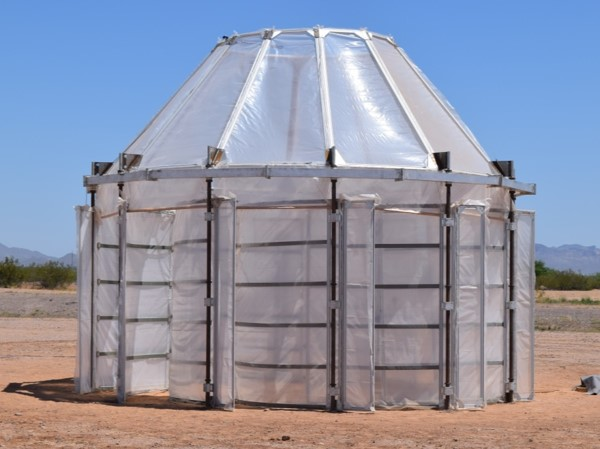
\includegraphics[width = 12 cm]{figs/sov_field}
    \caption{A photo of the field configuration, during the June 2015
    Field Test.}
    \label{fig:field_real}
   \end{center}
  \end{figure}

\subsection{Thermal Only}

While ambient winds in the field do impact system performance, it is
also illuminating to consider an idealized scenario with natural convection
driven only by thermal instabilities. Investigating this baseline,
thermal-only flow is intended to optimize the SoV apparatus to form a
strong thermal plume even in the absence of wind. After a system is
engineered to form a strong thermal plume, we can investigate to ensure
that the existing thermal vortex will be strengthened by the addition of
winds. \todo{do I need image of vanes? and explain how calculated}

\begin{figure}[htb]

 \begin{subfigure}{.55\textwidth}
  \centering
  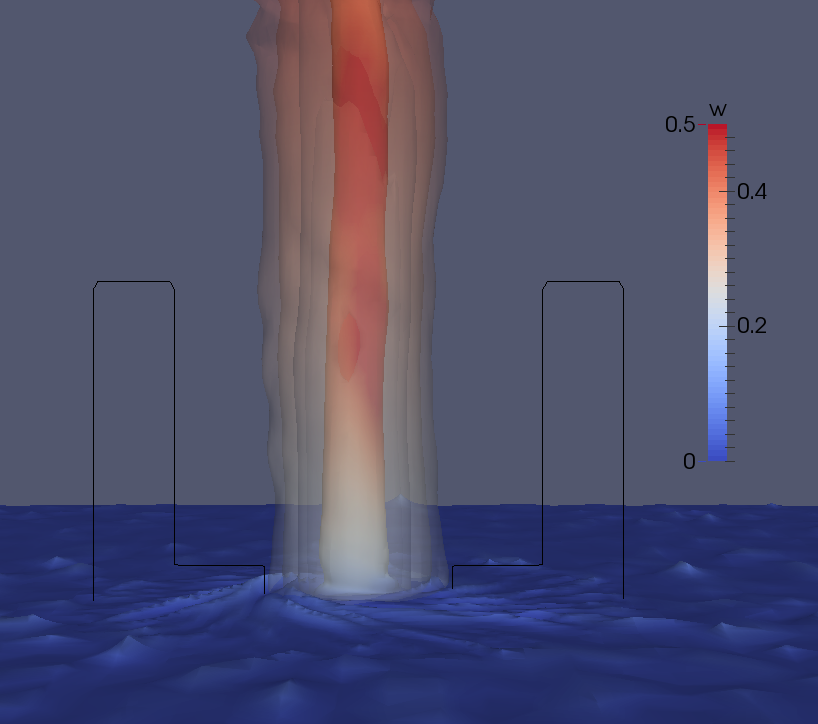
\includegraphics[width =0.7\textwidth]{figs/3d}
  \caption{Isocountours of the inner thermal core
  visible through semi-transparent contour around azimuthal velocity,
  colored by vertical velocity. }
  \label{fig:thermal}  
 \end{subfigure}%
 \begin{subfigure}{.4\textwidth}
  \centering
  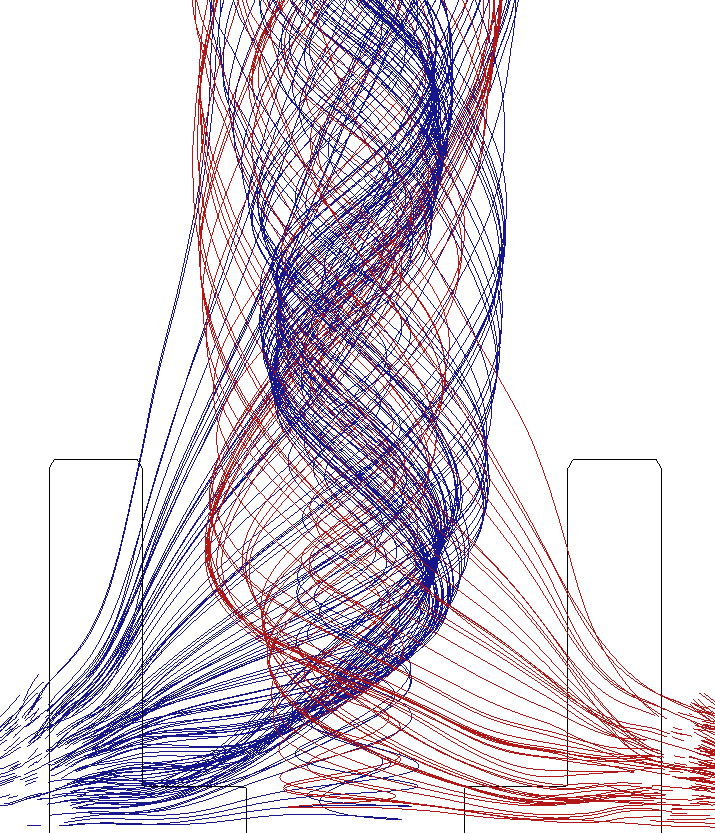
\includegraphics[width =0.8\textwidth]{figs/entrainment}%
  \caption{Fluid entrainment around the apparatus.} 
  \label{fig:entrain}  
 \end{subfigure}%
\end{figure}

In this subsection we show a representative case of an optimized thermal-only SoV
configuration. The results shown are the averages of several snapshots
from the field written over the course of several minutes. In general,
the averaging times are on the order of 20-30 wash-out times, where a
wash-out is defined as the time required for a particle at the base of
the apparatus to flow out through the top boundary. The energy flux
through the top of the vanes is roughly 53 watts. The solution
demonstrates several features characteristic of naturally occuring dust
devils. Figure \ref{fig:thermal} shows that we have formed a tight,
coherent thermal plume roughly the same size as the inner diameter of the
lower vanes. As anticipated, this hot flow is acting like a chimney,
generating a large vertical velocity which in turn entrains and draws in
outside flow. An image of the entrainment is shown in figure
\ref{fig:entrain}. The image was created by seeind particles advancing
them through the velocity field, showing the velocity field. One can
observe a tight inner vortex with significant azimuthal velocity formed
through the bottom tier of vanes, as well as a broader region of
entrained fluid through the second tier. 

\begin{figure}[htb]

 \begin{subfigure}{.5\textwidth}
  \centering
  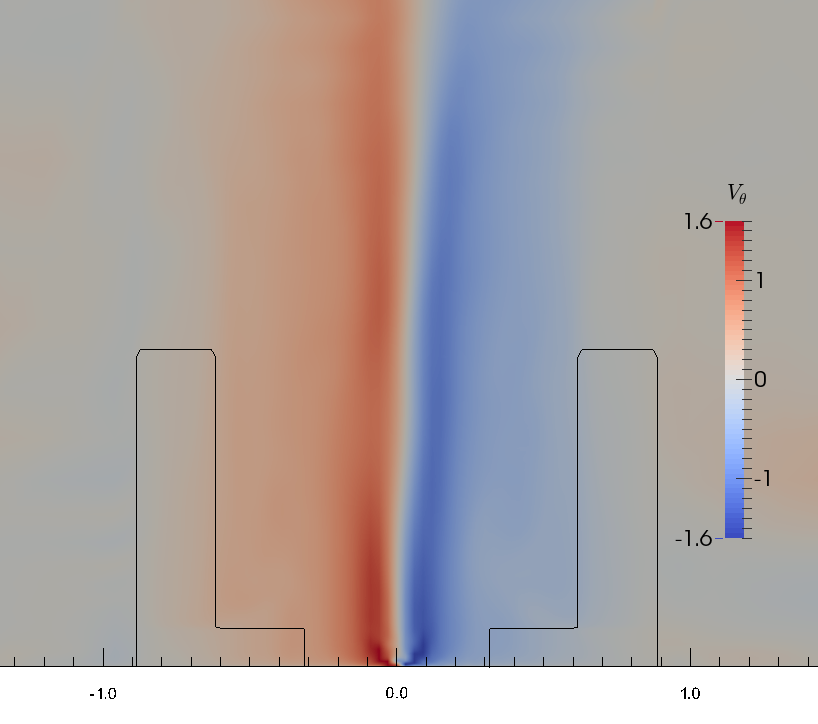
\includegraphics[width=.75\linewidth]{figs/vt}
  \caption{Azimuthal Velocity}
  \label{fig:vt-to}
 \end{subfigure}%
 \begin{subfigure}{.5\textwidth}
  \centering
  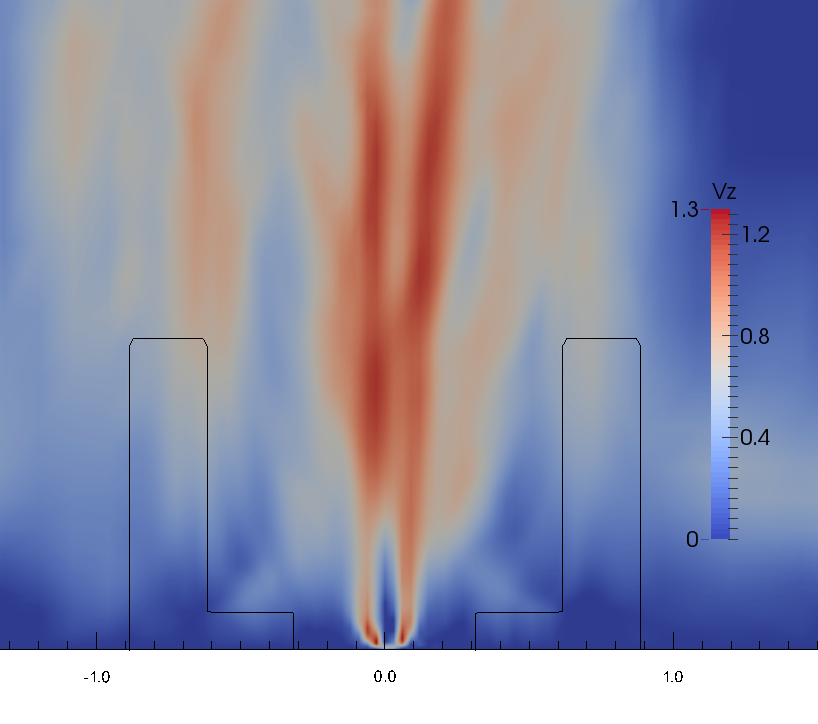
\includegraphics[width=.8\linewidth]{figs/vz}
  \caption{Vertical Velocity}
  \label{fig:vz-to}
 \end{subfigure}%


 \begin{subfigure}{.5\textwidth}
  \centering
  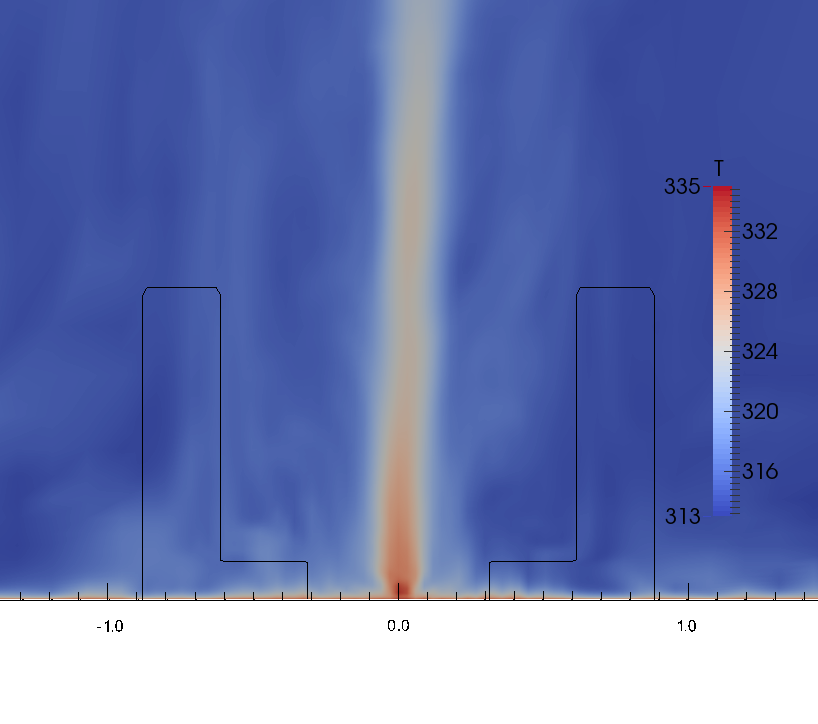
\includegraphics[width=.85\linewidth]{figs/t}
  \caption{Temperature}
  \label{fig:t-to}
 \end{subfigure}%
 \begin{subfigure}{.5\textwidth}
  \centering
  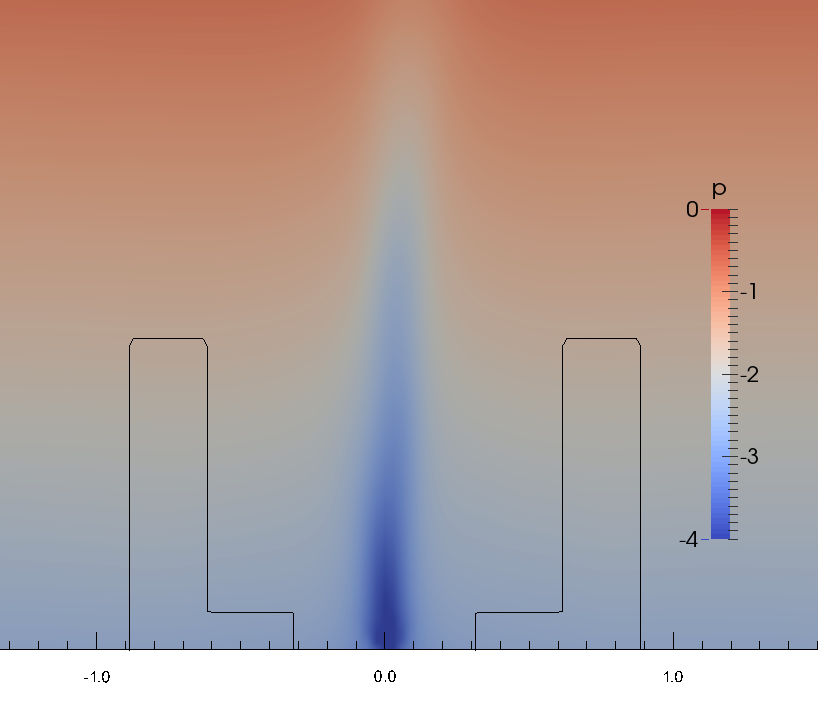
\includegraphics[width=.75\linewidth]{figs/p}
  \caption{Pressure}
  \label{fig:p-to}
 \end{subfigure}%

 \caption{Vertical slices for the thermal-only cases.}
 \label{fig:to-vert}
\end{figure}

%
%
%
Figure \ref{fig:to-vert} depicts several vertical slices through the SoV
for various state variables. One can see that there is a tight core
vortex with azimuthal and vertical velocities of several meters per
second. The tight vortex region coincides with a high temperature, low
pressure core region. The rapidly rotating air near the center induces
a low pressure core, as observed in real dust devils.
On the vertical velocity plot, notice that a small
downward flow region has formed in the middle of the vortex. 


Rotating air induces low pressure core, as observed in:
Dust Devils
\begin{figure}[htb]

 \begin{subfigure}{.5\textwidth}
  \centering
  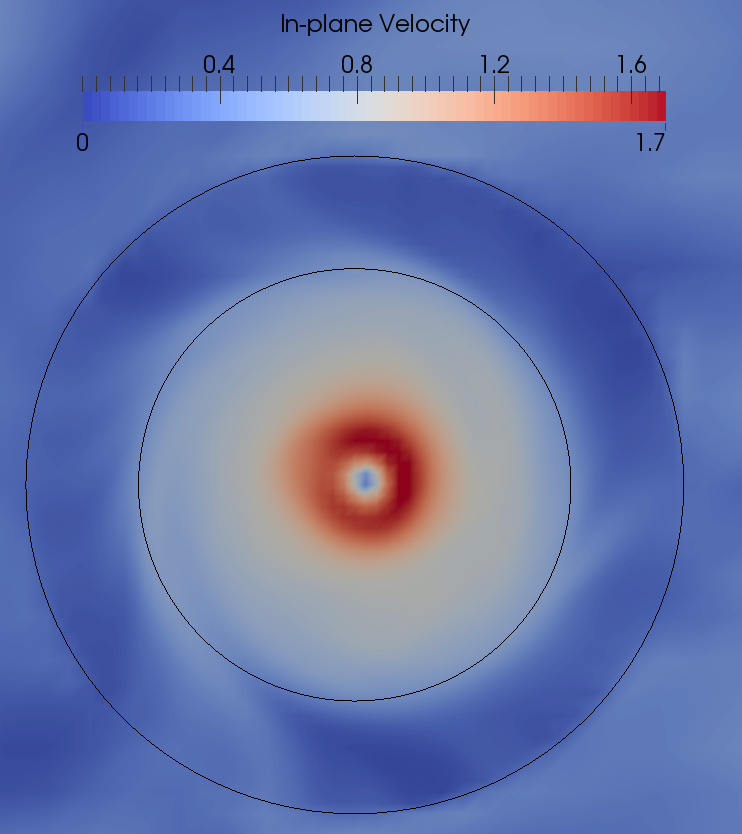
\includegraphics[width=.75\linewidth]{figs/vt_hor}
  \caption{Azimuthal Velocity}
  \label{fig:vt-to}
 \end{subfigure}%
 \begin{subfigure}{.5\textwidth}
  \centering
  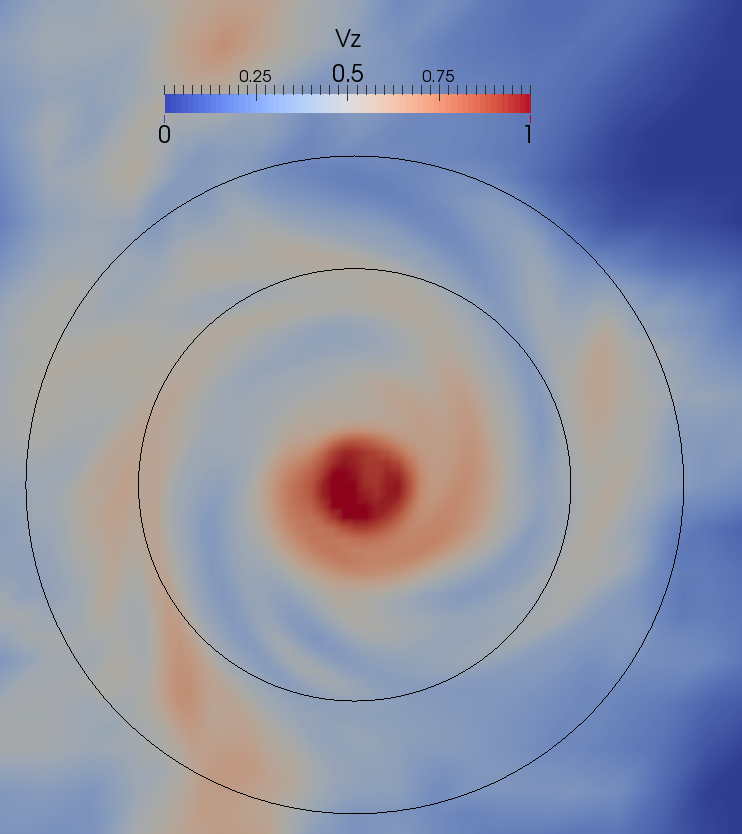
\includegraphics[width=.8\linewidth]{figs/vz_hor}
  \caption{Vertical Velocity}
  \label{fig:vz-to}
 \end{subfigure}%


 \begin{subfigure}{.5\textwidth}
  \centering
  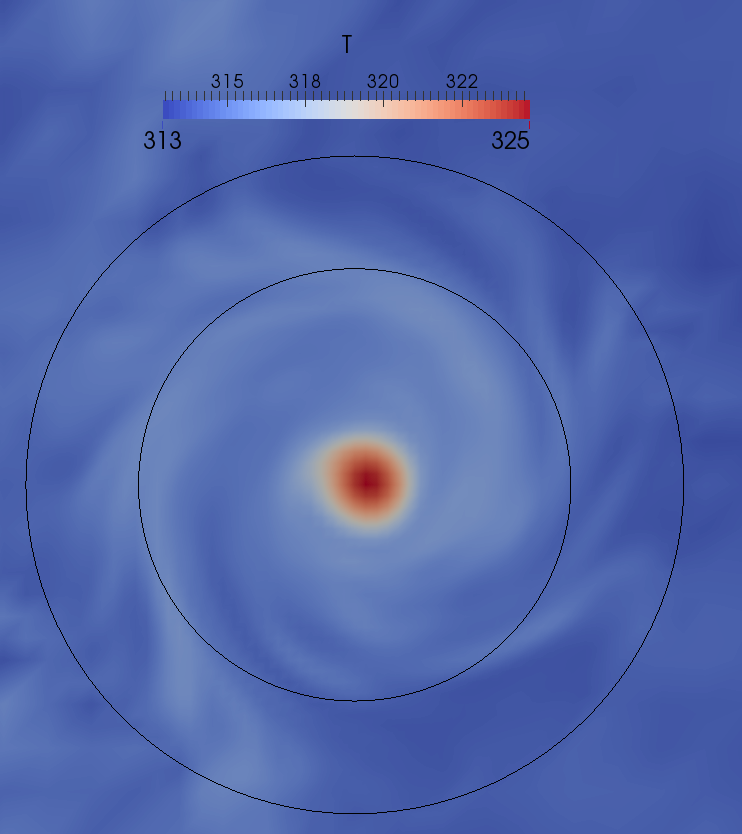
\includegraphics[width=.85\linewidth]{figs/t_hor}
  \caption{Temperature}
  \label{fig:t-to}
 \end{subfigure}%
 \begin{subfigure}{.5\textwidth}
  \centering
  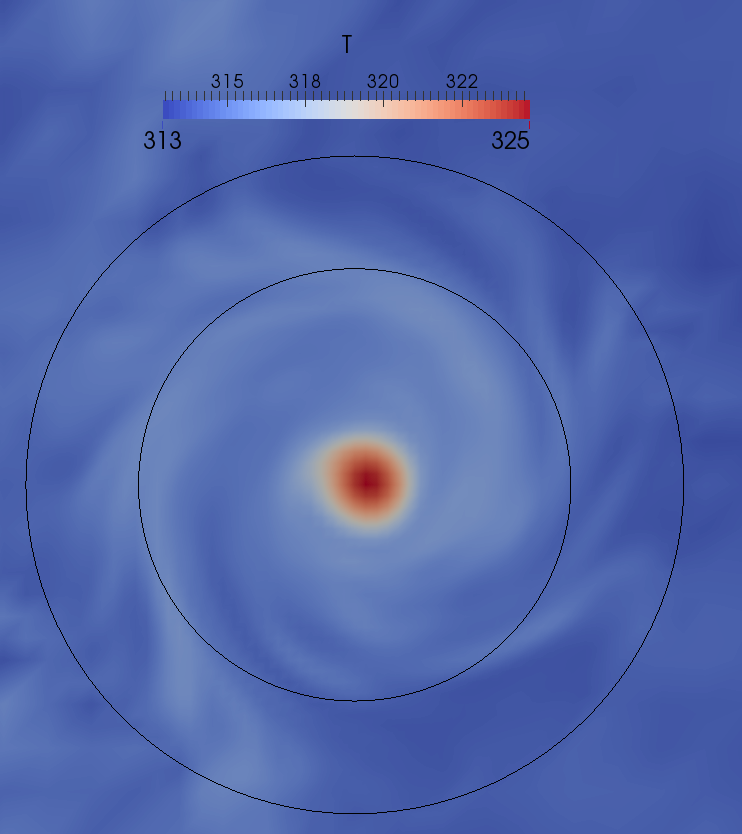
\includegraphics[width=.75\linewidth]{figs/t_hor}
  \caption{Pressure}
  \label{fig:p-to}
 \end{subfigure}%

 \caption{Horizontal slices for the thermal-only cases.}
 \label{fig:to-hor}
\end{figure}

Figure \ref{fig:to-hor}, in turn,  depicts several horizontal slices
through the SoV for the same state variables. It can be seen that the
large velocities are highly limited to a region just inside the
vanes. Likewise, the entrainment of fluid is limited to a region
immediately surrounding the vanes. 
%
% conclusion of thermal only
%
Finally, the thermal plume is relatively
narrow compared to the diameter of the device. It is desirable to
broaden the thermal plume, as this in turn creates a larger vertical
momentum flux due to the effects of buoyancy. This will presumably
entrain more surrounding fluid, driving it through the vanes and
imparting kinetic energy to the flow. The kinetic energy grows as the
square of the radius, so any broadening of the vortex core can greatly
enhance the kinetic energy flux. The diameter of the thermal core is
therefore a critical driver to the energy of the thermal-only
conditions, and operates as the ``prime-mover'' of the entire
process. Broadening this plume will necessarily enhance the energy
flux that can be extracted. However, the general physical
mechanisms that determine the thermal plume's thickness are not
presently understood. \todo{fix these images}
Regardless, these slices lend credibilty to the notion that our turning
vane configuration is generating something with parallels to a real dust 
devil.   

\subsection{Wind}



%
% horizontal slices
%
\begin{figure}[htb]

 \begin{subfigure}{.5\textwidth}
  \centering
  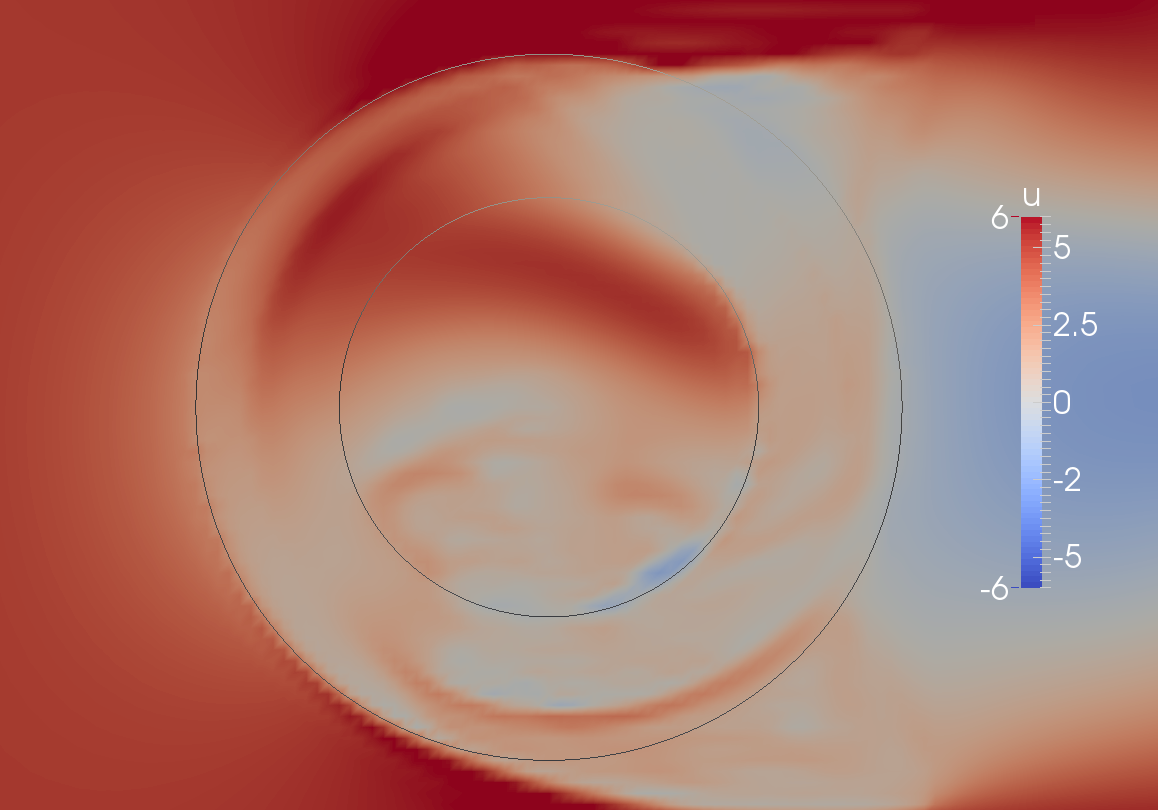
\includegraphics[width=.75\linewidth]{figs/wind_u}
  \caption{Streamwise}
  \label{fig:vt-wind}
 \end{subfigure}%
 \begin{subfigure}{.5\textwidth}
  \centering
  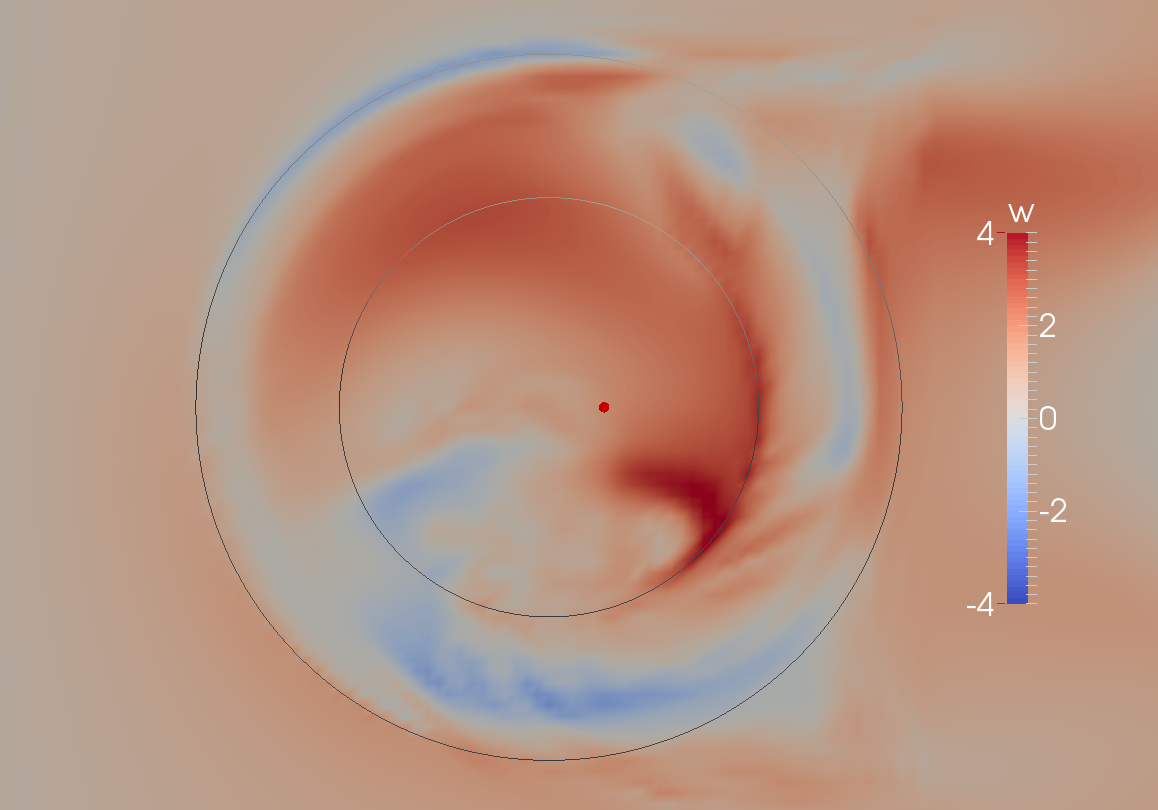
\includegraphics[width=.8\linewidth]{figs/wind_w}
  \caption{Vertical Velocity}
  \label{fig:vz-wind}
 \end{subfigure}%


 \begin{subfigure}{.5\textwidth}
  \centering
  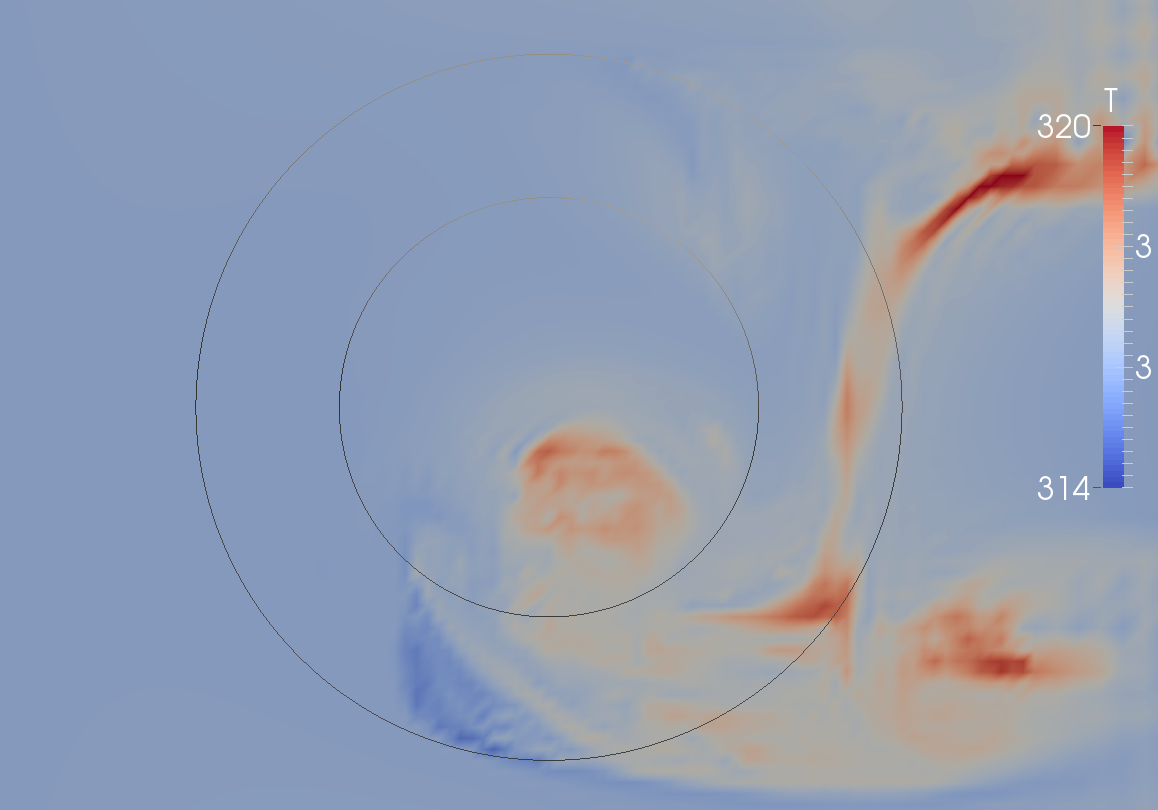
\includegraphics[width=.85\linewidth]{figs/wind_t}
  \caption{Temperature}
  \label{fig:t-wind}
 \end{subfigure}%
 \begin{subfigure}{.5\textwidth}
  \centering
  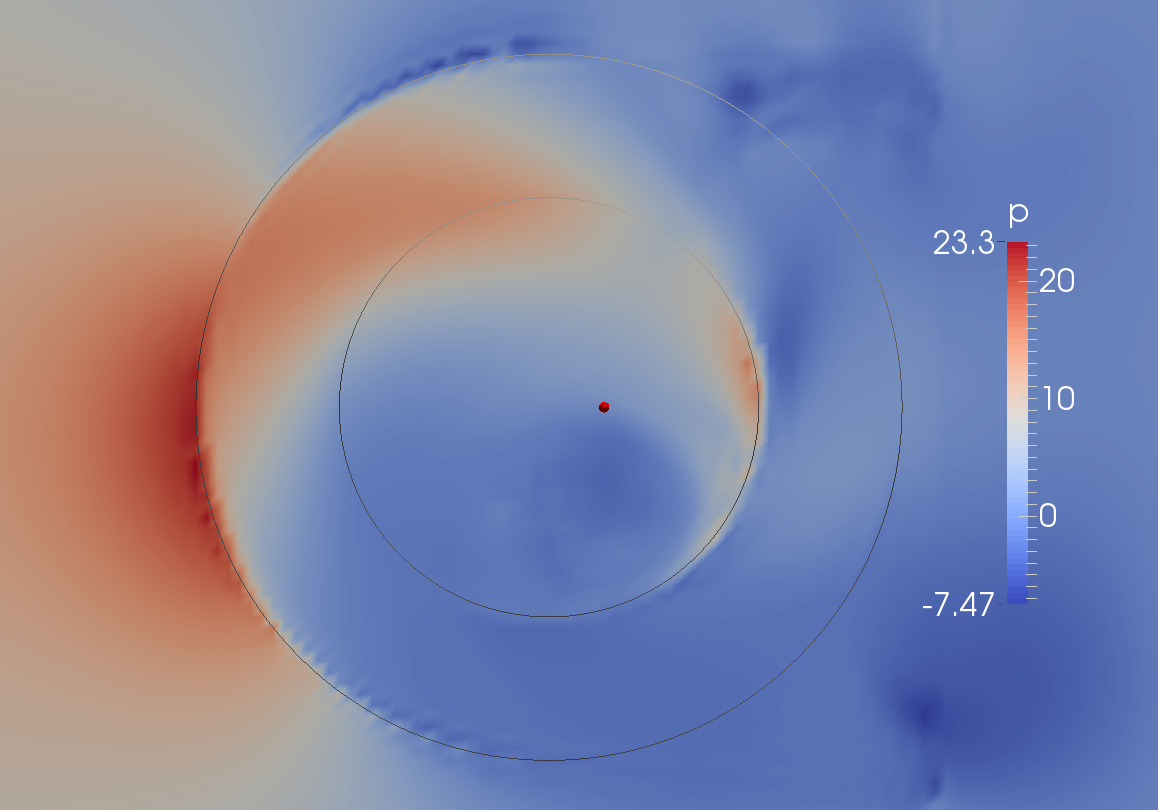
\includegraphics[width=.75\linewidth]{figs/wind_p}
  \caption{Pressure}
  \label{fig:p-wind}
 \end{subfigure}%

 \caption{Horizontal slices for the wind cases.}
 \label{fig:wind-hor}
\end{figure}

%
% vertical
%
\begin{figure}[htb]

 \begin{subfigure}{.5\textwidth}
  \centering
  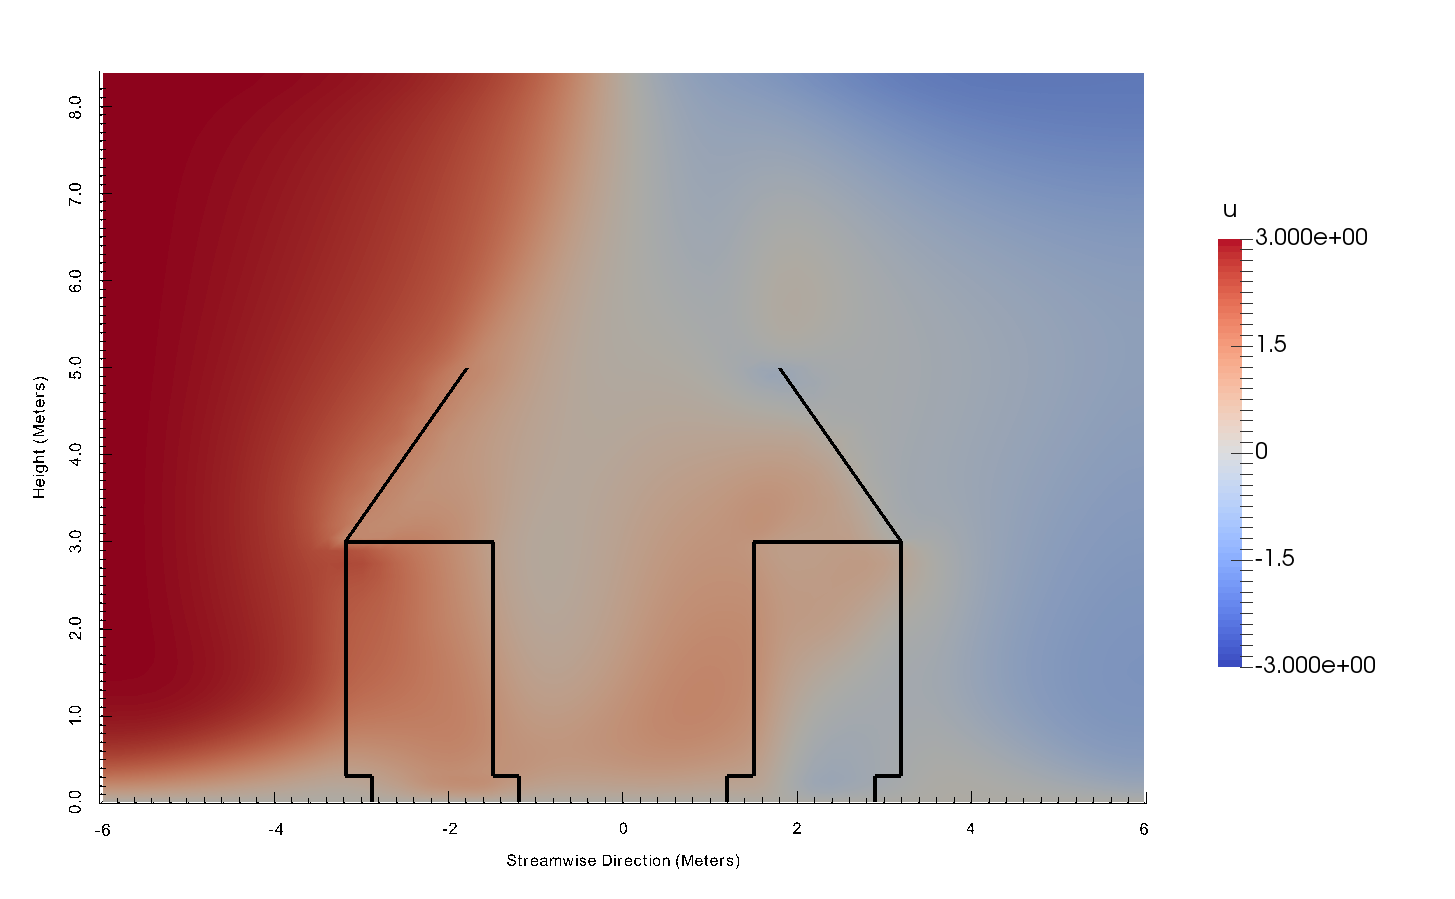
\includegraphics[width=.75\linewidth]{figs/wind_u_vertical}
  \caption{Streamwise}
  \label{fig:vt-wind-vert}
 \end{subfigure}%
 \begin{subfigure}{.5\textwidth}
  \centering
  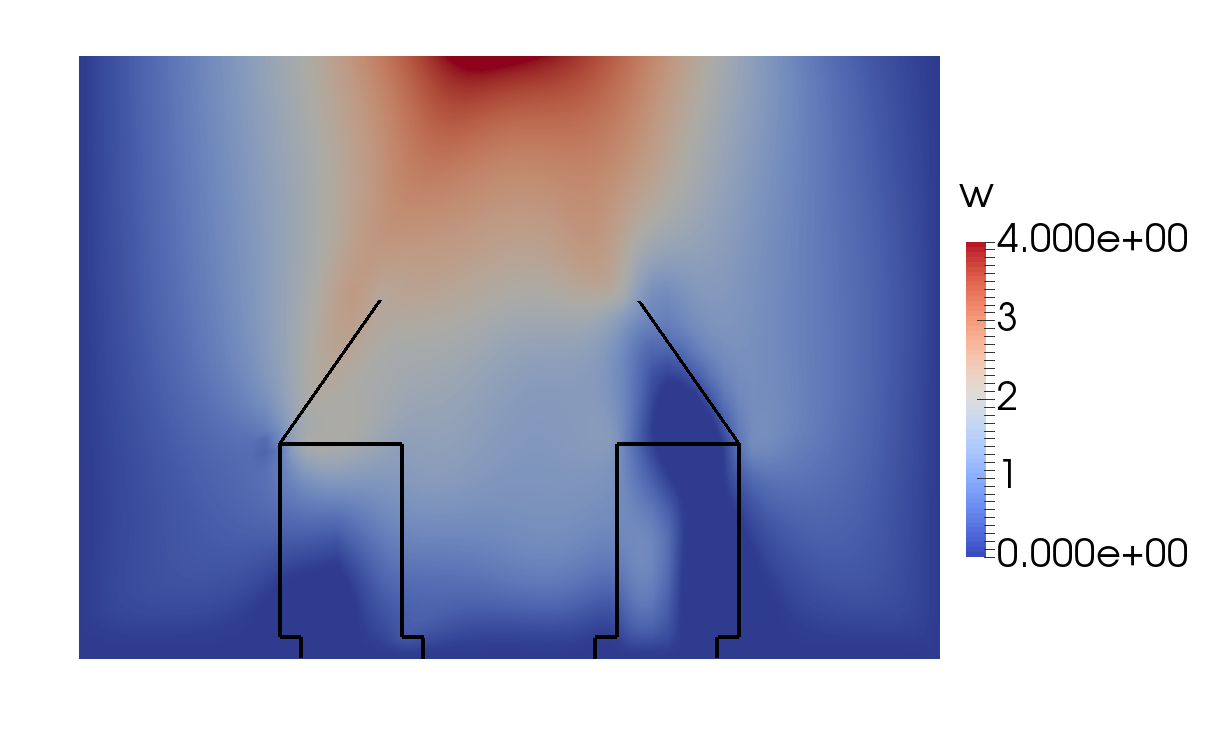
\includegraphics[width=.8\linewidth]{figs/wind_w_vertical}
  \caption{Vertical Velocity}
  \label{fig:vz-wind-vert}
 \end{subfigure}%


 \begin{subfigure}{.5\textwidth}
  \centering
  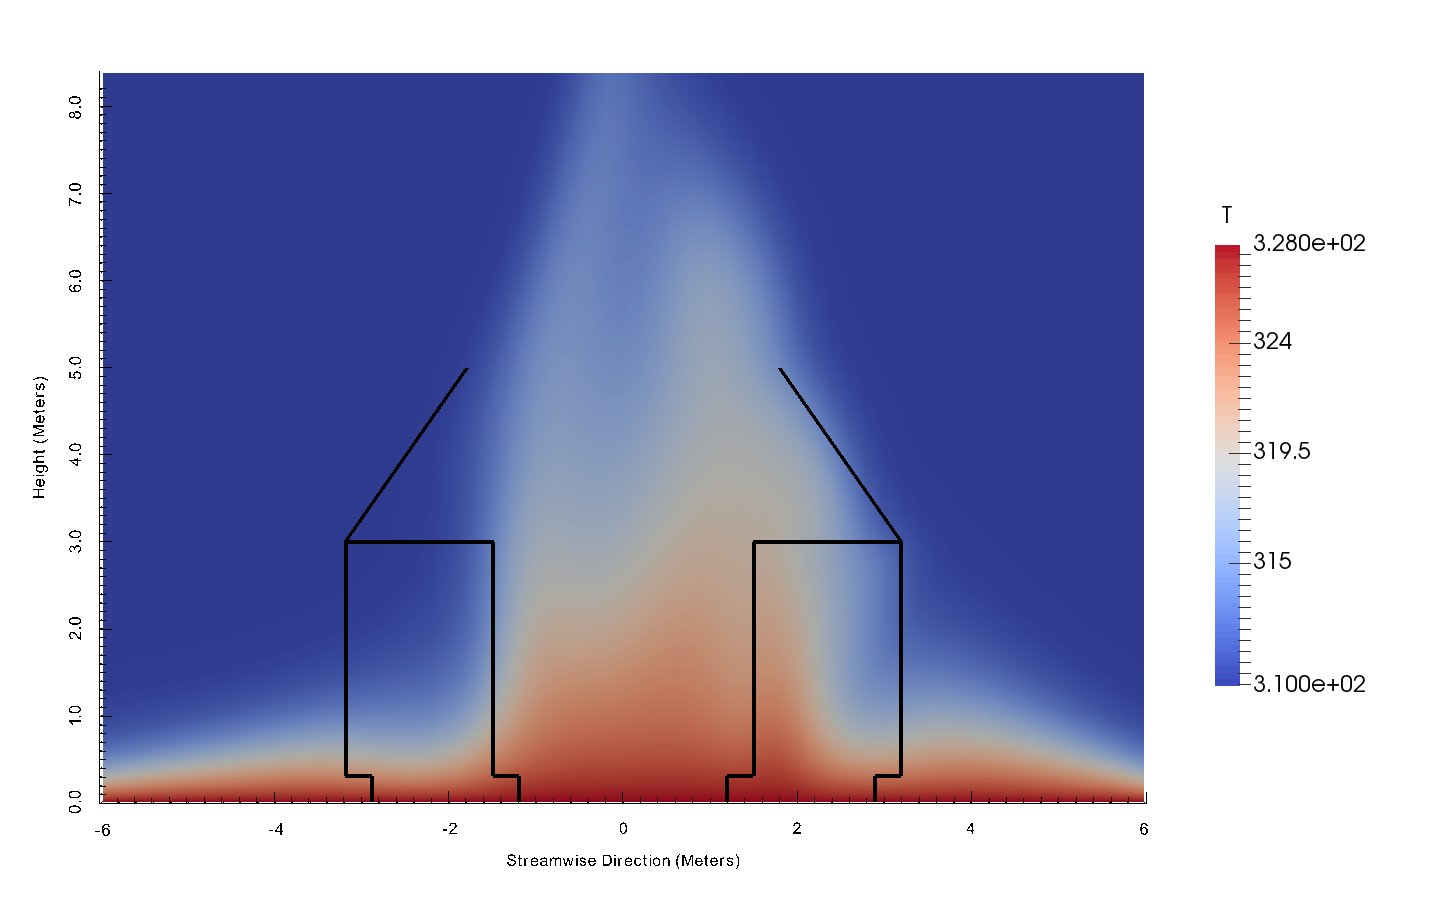
\includegraphics[width=.85\linewidth]{figs/wind_t_vertical}
  \caption{Temperature}
  \label{fig:t-wind-vert}
 \end{subfigure}%
 \begin{subfigure}{.5\textwidth}
  \centering
  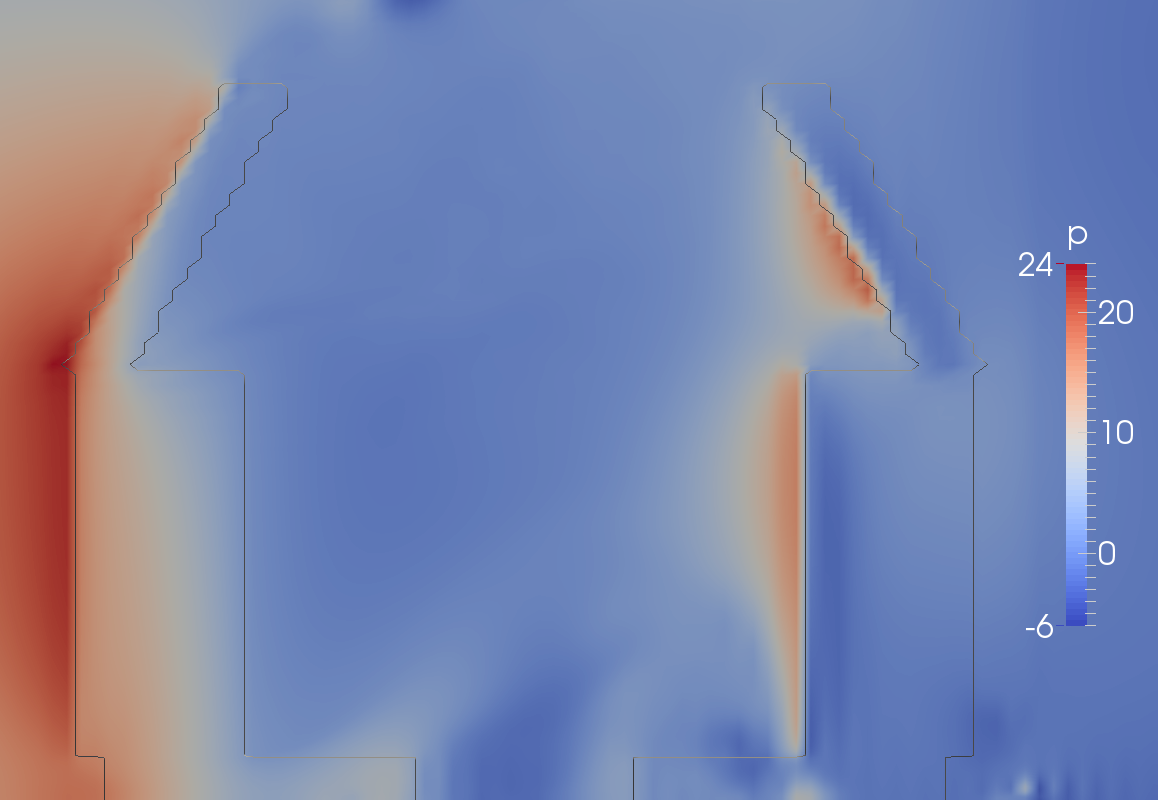
\includegraphics[width=.75\linewidth]{figs/wind_p_vertical}
  \caption{Pressure}
  \label{fig:p-wind-vert}
 \end{subfigure}%

 \caption{Vertical slices for the wind cases.}
 \label{fig:wind-ver}
\end{figure}

Observe that in all the plots, the thermal plume is significantly less
visible than in the thermal-only cases. While the
thermal-plume is necessarily weaker relative to the wind, some of this
is also due to the plume no longer being directly centered in the
flow. The plume is more visible using isocountors to render a
three-dimensional surface. Unlike the thermal-only, the flow in the wind
cases has a strong thermal gradient even exterior to the device. In
order to capture the difference between the ambient vertical temperature
and the warmer thermal plume, we use the potential temperature, defined
as, 
\begin{equation}
  \theta(x,y,z) = T(x,y,z) -T_{in}(z) 
   \label{eqn:theta}
\end{equation}
where $T_{in}$ is the proscribed inflow boundary temperature, described
in section \ref{sec:bc}. In this way the background potential
temperature is nearly zero, and larger values represent deviations from
the base flow temperature. The isocountour of a three Kelvin delta is 
depicted in figure \ref{fig:field_real}. This gradient was selected as
it was noted as sufficient for formation of a dust devil by
Sinclair\cite{Sinclair1969}. 

%
% t iso
%
  \begin{figure}[!htb]
   \begin{center}
    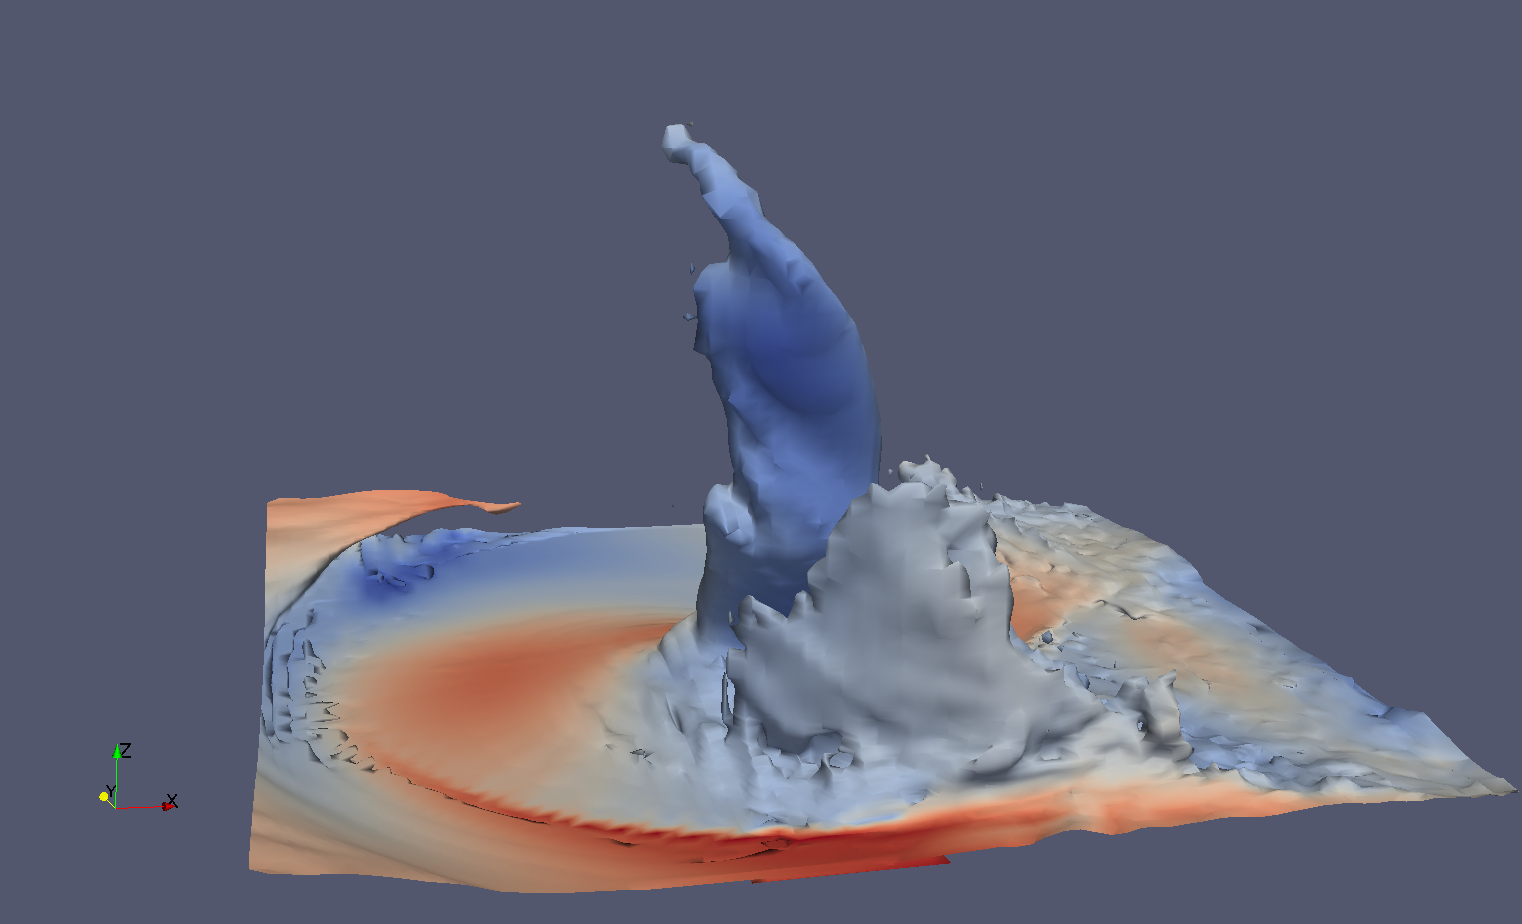
\includegraphics[width = 12 cm]{figs/t_iso}
    \caption{Isocountor of the Thermal Plume. Here, the isocontour is
    labelled by the potential temperature, $\theta$, as defined in \ref{eqn:theta}.}
    \label{fig:field_real}
   \end{center}
  \end{figure}

\subsection{Optimization}

In this section we show results from a representative optimization
effort for a thermal-only case, in order to detail the mode of operation
these efforts have presently followed. 

typical mode of scientific and engineering inquiry, which is to say
hypothesis of system operation followed by testing and then evaluation
and possibly, validation of the testing. 


Our principle quantity of interest (qoi) is the energy that we can
extract from the synthetic dust devil. As a surrogate to this quantity,
we consider the energy flux through a region near the top of the vanes,
where we expect to add a turbine that will be driven by the flow. The
flux here is the magnitude of energy passing in unit time through the
unit area pertpendicular to the direction of the velocity. This is a
simple path integral that has the form\cite{landau1959fm},  
\begin{equation}
 \dot E = -\oint \rho \textbf{v}(\frac{1}{2}v^2 + \epsilon) \cdot d \textbf{f}
\end{equation}
where $\epsilon$ is the internal energy. % and $d\textbf{f}$ the. 
For our problem, we consider an incompressible fluid flowing through a
flat horizontal region interior to the vanes in the x-y plane, which
results in, 
 \begin{equation}
 \dot E = -\frac{\rho }{2} \int V_z (V_{\theta}^2 + V_z^2 ) dA
 \end{equation}
This shows the energy each unit mass of fluid carries with it as it
moves through the defined surface. 

\begin{figure}[htb!]
 \begin{subfigure}{.5\textwidth}
  \centering
  
\includegraphics[width=.75\linewidth]{figs/before_vanes}
  \caption{Vanes before optimization}
  \label{fig:vt-wind-vert}
 \end{subfigure}%
 \begin{subfigure}{.5\textwidth}
  \centering
  
\includegraphics[width=.8\linewidth]{figs/after_vanes}
  \caption{Vanes after optimization}
  \label{fig:vz-wind-vert}
 \end{subfigure}%
\end{figure}


image of flow before after

\begin{figure}[htb!]
 \begin{subfigure}{.5\textwidth}
  \centering
  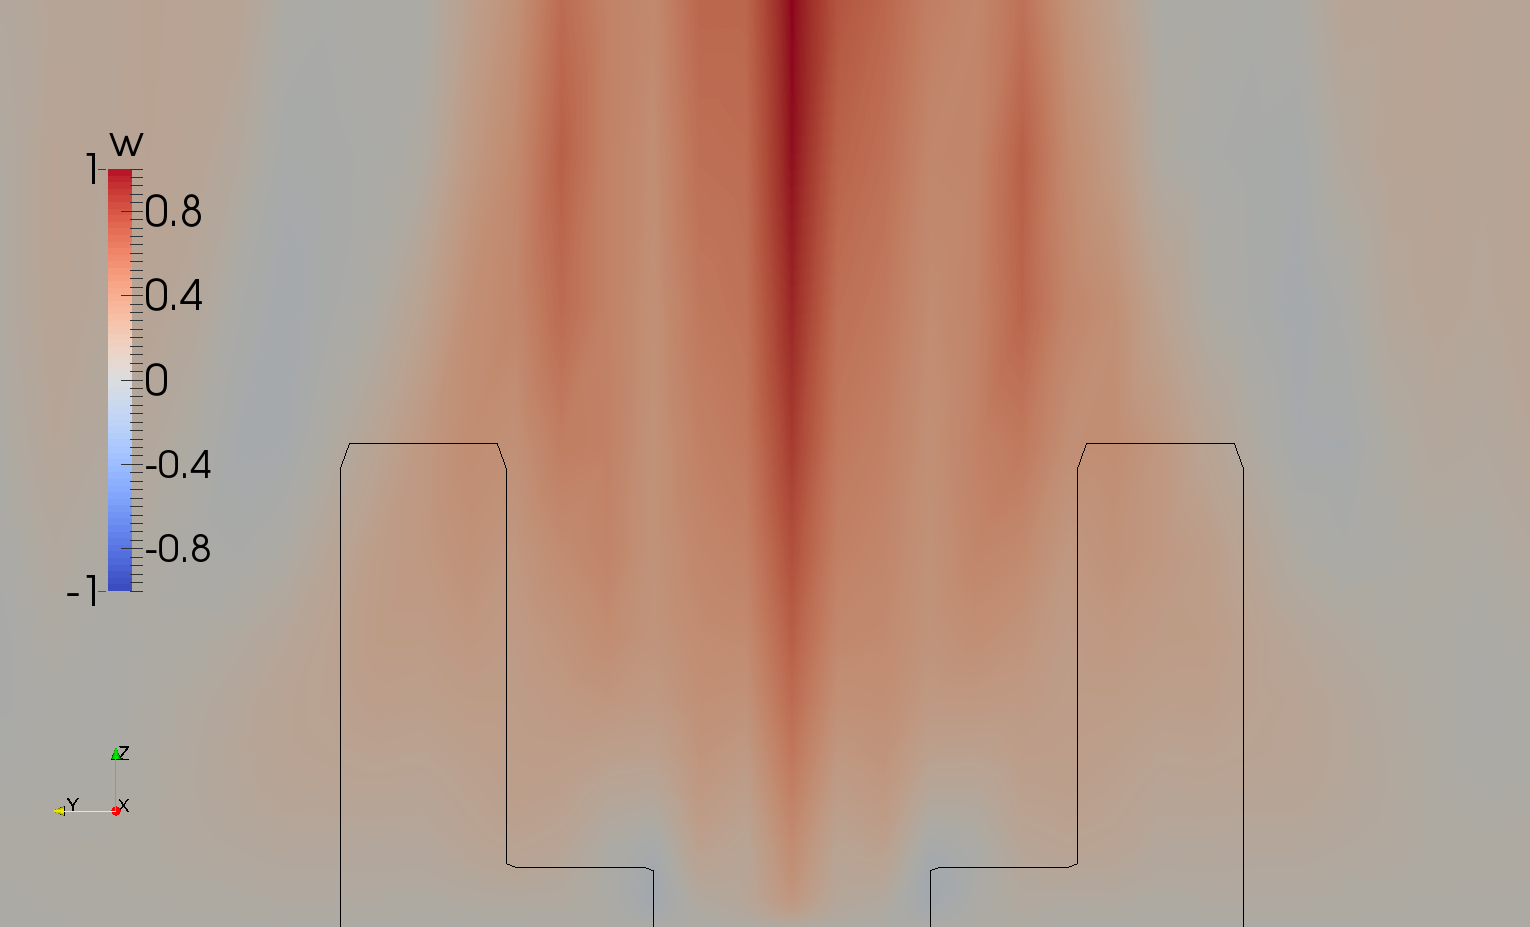
\includegraphics[width=.75\linewidth]{figs/before_opt}
  \caption{Flow before optimization}
 \end{subfigure}%
 \begin{subfigure}{.5\textwidth}
  \centering
  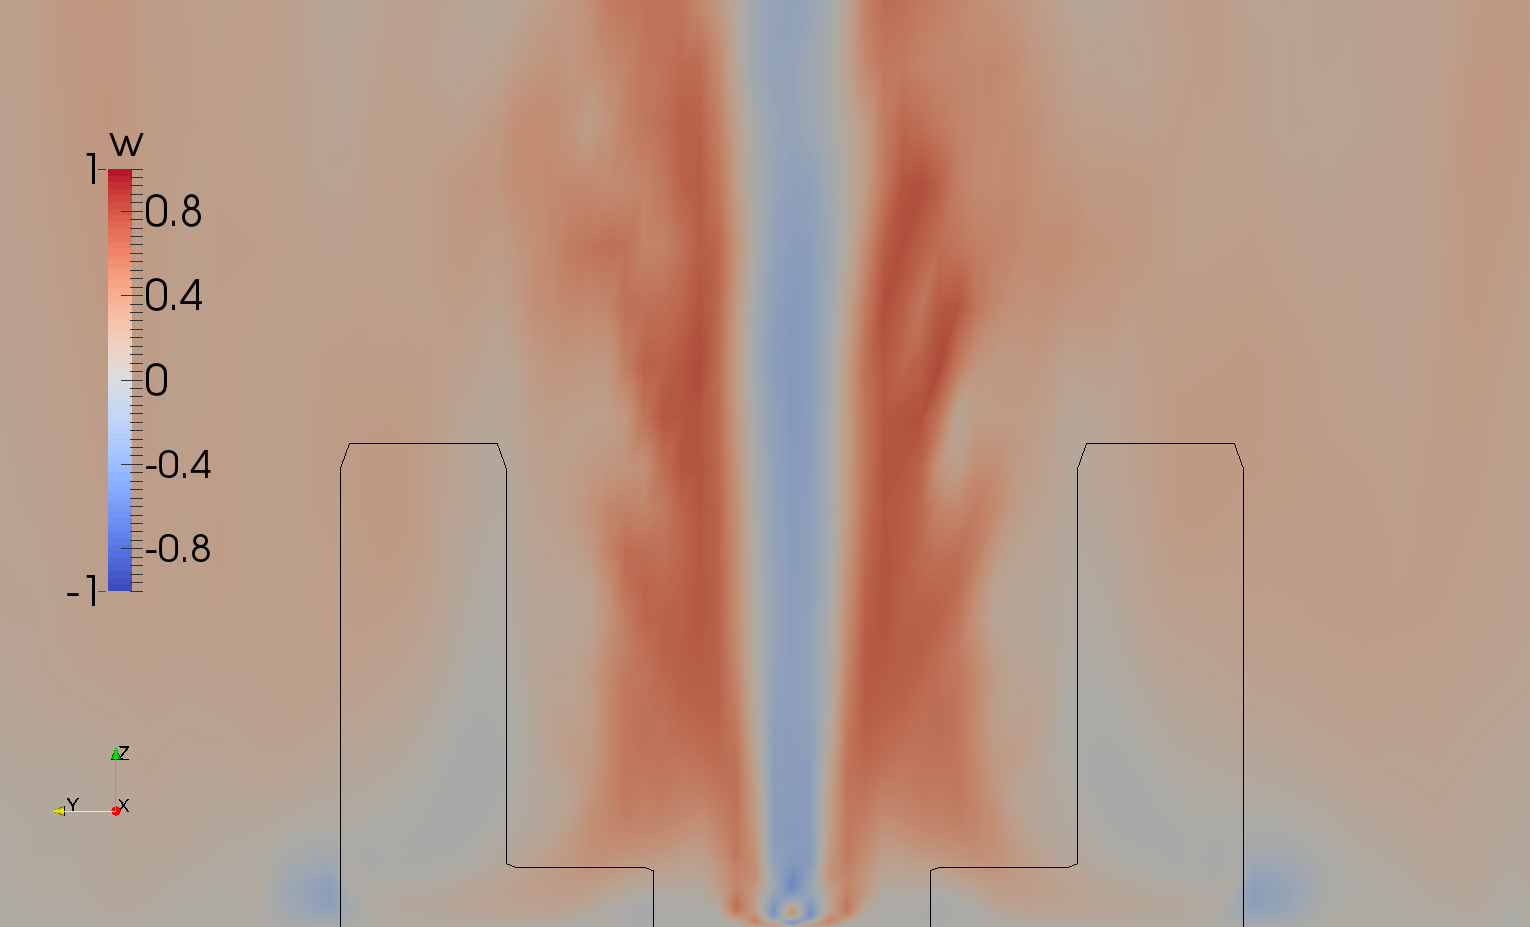
\includegraphics[width=.8\linewidth]{figs/after_opt}
  \caption{Flow after optimization}
 \end{subfigure}%
  \label{fig:opt_flow}
\end{figure}

table of energy flux increase

\begin{figure}[htb]
 \centering
 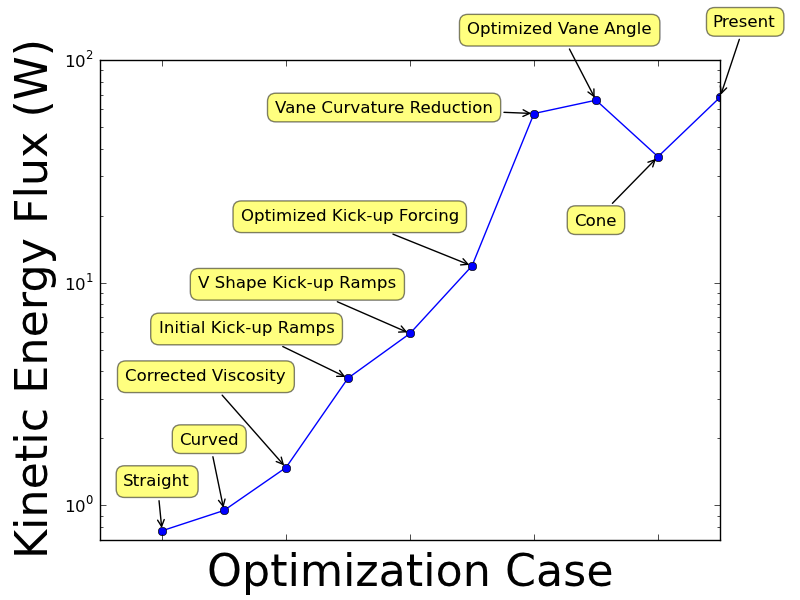
\includegraphics[width=.75\linewidth]{figs/opt_plot}
 \caption{Streamwise}
 \label{fig:opt_plot}
\end{figure}
